\chapter{Einleitung}

\section{Was ist ein RAG}

\begin{figure}[h!]
    \centering
    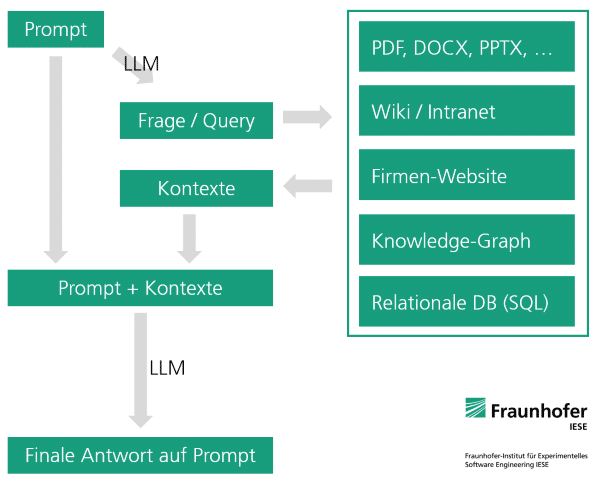
\includegraphics[width=0.5\textwidth]{retrieval_augmented_generation_RAG_600px.png}
    \caption{Struktur eines RAGs, Quelle: \cite{honroth2024retrieval}}
    \label{fig:Rag Structure}
\end{figure}

\begin{quote}
    Bei Retrieval Augmented Generation (RAG) erweitert man den Prompt für das LLM um Suchergebnisse aus einer Dokumentensammlung, einer Datenbank, einem Wissensgraf (Knowledge Graph) oder einer anderen Suche (z.B. Internetsuche). Das Wissen für die Antwort kommt also aus angebundenen Quellen und nicht aus dem LLM.
\end{quote}
\cite{honroth2024retrieval}\\ \\

\subsection{Warum ein RAG}
Wenn es darum geht, Wissen abzurufen, haben LLMs zwei Probleme.

Wissen, welches nur selten im Training erwähnt wurde, können selbst die größten LLMs nicht lernen.
Das zweite Problem ist, dass LLMs einen gewissen Wissensstand haben und weiter trainiert werden müssen, um die neuesten Informationen zu kennen.
% TODO: Proper citations needed for these claims
% https://aclanthology.org/2023.acl-long.546/
% https://arxiv.org/abs/2211.08411

Die Nutzung eines RAGs ist eine der beiden Möglichkeiten, um ein LLM zu verbessern. Die andere Möglichkeit ist das Finetuning des LLMs. Es gibt jedoch wichtige Unterschiede zwischen diesen beiden Methoden.

Es gibt einige Faktoren, welche die Entscheidung beeinflussen können, ob ein RAG oder ein Finetuning besser für den betrieblichen Ablauf geeignet ist.

\subsection{Kompetenz}
Beim Finetuning ist ein gewisses technisches Wissen notwendig, um die Themen Natural Language Processing (NLP), Deep Learning, Modellkonfiguration, Datenaufbereitung und Evaluierung anzuwenden.
Der gesamte Prozess des Finetunings ist sehr komplex und erfordert viel Zeit und Ressourcen.

\subsection{Art der Daten}
Sollten die Daten dynamisch sein, ist das RAG die bessere Lösung, da es die Daten schneller und kontinuierlich aktualisieren kann.
Der Prozess des Finetunings erstellt immer eine Momentaufnahme, die ein erneutes Training erfordert.
Beim Finetuning ist es möglich, dass das Modell Muster erkennt und firmeneigene Begriffe verstehen kann.

\subsection{Budget}
Das Finetuning erfordert teure Rechenzeit auf Hochleistung-GPUs, was das Training eines Modells sehr teuer macht.
Das RAG hat dagegen zusätzliche Kosten, die durch das Speichern der Daten in einer Vektordatenbank entstehen.


\section{Objektive Beurteilung von RAGs}
Je mehr Daten einem RAG zur Verfügung stehen, desto aufwendiger ist es, die Qualität des RAGs zu beurteilen.
Eine Beurteilung durch Menschen müsste bei Anpassungen am RAG oder Änderungen an den Daten immer wieder neu durchgeführt werden.
Menschliche Beurteilungen sind teurer, daher ergibt es Sinn, mithilfe von LLMs die Beurteilung zu automatisieren.
Es gibt bereits Tools wie RAGAS, die versuchen, diesen Prozess unter anderem mithilfe von LLMs zu automatisieren.
Diese Tools generieren aus den ihnen gegebenen Daten Fragebögen, die auf eine Frage eine beispielhafte Antwort und die genutzten Stellen aus den vorher gegebenen Dokumenten beinhalten.
Sollten nach diesem automatisierten Test die gewünschten Ergebnisse nicht erreicht werden, kann zum Beispiel die Veröffentlichung blockiert werden.

Sowohl menschliche Bewertungen als auch die reine subjektive Bewertung durch LLMs sind nicht objektiv.
Mithilfe von mehreren Techniken kann versucht werden, die Bewertung mithilfe von LLMs objektiv zu machen.

\section{Darstellung des Themas und der Forschungsfragen}
In dieser Bachelorarbeit wird untersucht, wie gut diese Tools sowohl subjektive als auch objektive Bewertungen durchführen können.
Im Mittelpunkt werden die beiden Tools RAGAS und Giskard stehen, welche die Bewertung durchführen.




\section{Praxistauglichkeit und Herausforderungen}
Es stellen sich mehrere Herausforderungen für die Bewertung von RAGs durch diese Tools.
Die erste sind die Kosten, die bei der Bewertung entstehen. Für die Bewertung muss das neue System, welches getestet wird, aufgesetzt werden.
Dies beinhaltet eine eventuelle doppelte Speicherung der Daten und die für das Testen benötigten Aufrufe des LLMs.
Neben den Kosten ist auch die Zeit, welche es dauert, die Bewertung durchzuführen, relevant, da die Bewertung schneller durchgeführt werden kann, wenn mehr Ressourcen zur Verfügung stehen.
Das System muss auch auf dem neuesten Stand gehalten werden, da sich dieses noch relativ junge Thema schnell entwickelt.

Content filtering

\section{Softwaretechnische Fragestellungen}

In dem Artikel \textit{RAG in der Praxis – Generierung synthetischer Testdatensätze} von Luka Panic~\cite{pixion2024rag} treten Fehler beim Generieren der Testfragen auf. 17\% ist hier die Fehlerquote.
Dies hat vielfältige Gründe, die von nicht verwertbaren Antworten des LLMs bis zu Verbindungsproblemen oder dem Erreichen des Limits der maximalen Anfragen an APIs reichen.

Auch bei der Bewertung von Antworten können sich ungewollte und bisher noch ungeahnte Biases einschleichen. In diesem Paper \cite{yang2023llmfairness} wird gezeigt, dass, wenn ein LLM eine von zwei gegebenen Antworten aussuchen müsste, die erste bevorzugt wurde, selbst wenn die gleiche Frage mit anderer Reihenfolge gestellt wurde.
RAGs vergleicht keine Antworten miteinander und daher ist dieser Bias kein direktes Problem für uns. Was jedoch einen Einfluss auf die Bewertung von Antworten haben kann, ist der Bias zu gewissen Nummern.
Wie in \cite{shaikh2024cbeval} beschrieben, bevorzugen LLMs bei der Bewertung lieber Zahlen, welche Mehrfache von 5 und 10 sind.

Auch die allgemeine stochastische Natur von LLMs spielt eine Rolle, da bei der gleichen Anfrage unterschiedliche Antworten und dadurch auch Bewertungen zurückgegeben werden. Wie groß diese Abweichungen sind, wird in dieser Arbeit kurz untersucht.

Wie in diesem Paper \cite{gemini2024v15} beschrieben, stellt Gemini 1.5 einen bedeutenden Fortschritt in der multimodalen Verarbeitung großer Kontextfenster dar. Das wirft auch die Frage auf, ob RAGs nicht irrelevant sind und durch LLMs mit großen Kontextfenstern abgelöst werden.
Es gibt einige Gründe, die dagegen sprechen: LLMs mit größeren Kontextfenstern werden immer langsamer und teurer, die genauen Kosten sind abzuwarten. Jedes Mal alle Daten in den Kontext zu laden, besonders wenn dies über das Internet geschieht, ist eine weitere Hürde. LLMs fällt es auch schwer, bei zu vielen Informationen noch die relevanten zu finden, was zu schlechteren Antworten führen kann.
Diese Faktoren lassen darauf schließen, dass RAGs, die nicht nur eine einfache Suche nutzen, noch länger relevant bleiben.

Kann ich hier wirklich Diskussionen von Twitter linken oder mache ich mich dann lächerlich?
https://x.com/agishaun/status/1758561862764122191
https://x.com/ptsi/status/1758511315646320920


Pitfalls in LLM Assisted Evaluation https://medium.aiplanet.com/evaluate-rag-pipeline-using-ragas-fbdd8dd466c1
